\chapter{Lineær programmering}

\begin{comment}
Ting til retter
- bør "def 5.5 mulige løsninger og den mulige mængde" komme før "standard maksimums- og minimumsproblemer"? %Nej, det synes jeg ikke
- Jeg er ikke sikker på alle termer i dette afsnit. Jeg rettede kriteriefunktion til objektfunktion, da der blev brugt objektfunktion i projektforslaget.
- Jeg er lidt inkonsistent med anvendelsen af [1 2 3] og [1,2,3]. er ikke helt sikker på hvad der ser bedst ud. %Hvis det er en vektor så er det [1 2 3]
- Er der brug for at skrive betingelserne og objektfunktionen ud i starten, eller er det nok at det skrives som vektor-vektor produkt?
\end{comment}

Lineær programmering er en anvendelse af lineær algebra til at løse et optimeringsproblem. Lineære programmeringsproblemer tager udgangspunkt i maksimering eller minimering af en lineær funktion. For variablene er der fastsat en række af betingelser, som begrænser de mulige løsninger til problemet.
%Ved ikke: Må vi antage at læseren ved, hvad en lineær funktion er, for tror de ikke bare at det er ax +b?


Funktionen, som ønskes optimeret, kaldes \textbf{objektfunktionen}, og findes på formen:
\begin{align}
f(\vec{x})\ = \vec{c}^T \vec{x} \ =  c_1x_1 + c_2x_2 + \cdots + c_nx_n,
\end{align}
hvor $\vec{x}= \rvect{x_1 & x_2 & \cdots & x_n}^T$ og $\vec{c}= \rvect{c_1 & c_2 & \cdots & c_n}^T$.

\begin{comment}
Bør muligvis være en defintion, behøver ikke at skrives ud, men så skal f(\vec{x}) frem for f(x_1, ..., x_n).  Men det er jo variable repræcenteret ved en vektor så måske introducerer f(x_1, ..., x_n), udenfor definitionen.
\begin{defn}
Betragt et lineært programmerings problem, da er \textbf{objektfunktionen}
\begin{align*}
f(\vec{x}) = \vec{c}^T \cdot \vec{x}, 
\end{align*}
for $\vec{x}, \vec{c} \in \mathds{R}^n$, funktionen, som ønskes optimeret.
\end{defn} Eller noget, det er vigtigt at denne definition, vil kræve at vektor x og c bliver introduceret i den bindende tekst.
\end{comment}


%hvis objektfunktionen defineres, så bør det samme ske for bibetingelserne.
Dertil tilføjes en række af betingelser for variablene. Betingelser på formen
\begin{align}
	x_i \geq 0,
\end{align}
kaldes \textbf{positivitetsbetingelser}.
Andre lineære betingelser for variablene kaldes for \textbf{lineære bibetingelser}, og findes på formen, 
\begin{align}
	a_{i,1} x_1 + a_{i,2} x_2 + \cdots + a_{i,n} x_n \  = \ \vec{a}_i^T\vec{x} \ (\leq,=,\geq) \  b_i, \quad \text{for} \ i \in \{1,2,\cdots, m\}, %Kan man bruge \leq,=,\geq)?
\end{align}
hvor $m$ er antallet af lineære bibetingelser. I en lineær bibetingelse kan venstresiden være begrænset med $\leq, \geq$ eller $=$ i forhold til højresiden. I nogle typer af programmeringsproblemer anvendes kun en enkelt af disse relationer. Positivitetsbetingelser er et specialtilfælde af de lineære bibetingelser, da en positivitetsbetingelse, $x_i \geq 0$, blot kan ses som en lineær bibetingelse, hvor en koefficienten til $x_i$ er 1, mens resten af koefficienterne er 0 og hvor $b_i=0$.

En \textbf{mulig løsning} er en vektor $\vec{x}$, som overholder alle problemets betingelser. %Bør nok skrives som en definition, men det kan være at det først skal ske under geo? Bertimaz har i hvertfald en strangent def.

Et eksempel på et lineært programmeringsproblem ses i Eksempel \ref{eks:maksprob1}. Eksemplet er et lineært maksimeringsproblem, da objektfunktionen ønskes maksimeret.

\begin{eks}
Et eksempel på et lineært programmeringsproblem ses her, hvor funktionen $f(x_1,x_2)=4x_1+3 x_2$ skal maksimeres.
\begin{center}
\begin{tabular}{l	>{$}r<{$}	>{$}r<{$}	>{$}l<{$}}
Maksimer 		& 		4x_1&	+3 x_2	& \\
med hensyn til 	&  \ \ 	2 x_1& 	- 4 x_2	& \geq - 8\\
				&  		x_1& 	+3 x_2	& \leq 16\\
				&  \ \ 	x_1& 			& \leq 10\\
og $x_1,x_2\geq 0$
\end{tabular}
\end{center}


%Mængden af alle mulige løsninger til problemet kan vises grafisk. De mulige løsninger findes inden for det grå område på Figur \ref{fig:maksprob1}, hvor $x_1$ og $x_2$ vises henholdsvis på 1. og 2. aksen. %Hvor får du det grå område fra?
%
%\begin{center}
%	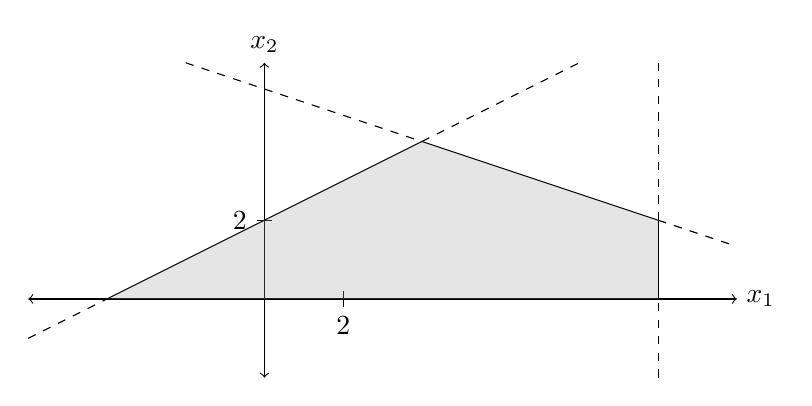
\begin{tikzpicture}
  %laver Grid
  	%\draw[thin,gray!40] (-3,-1) grid (6,3); 
  %x-aksen
  	\draw[<->] (-3,0)--(6,0) node[right]{$x_1$}; 
  %y-aksen
  	\draw[<->] (0,-1)--(0,3) node[above]{$x_2$};
  	
  %akse-markeringer
  	%\node[left] (xakse) at (0,1) {2};
  	\draw[] (-0.1,1) -- (0.1,1) node[pos=0,left] {2};
  	\draw[] (1,-0.1) -- (1,0.1) node[pos=0,below] {2};
  	
  %ligning 1
	\draw[domain=-3:-2,variable=\x,dashed] 	plot({\x},{0.5*\x+1});
	\draw[domain=-2:2,variable=\x] 			plot({\x},{0.5*\x+1});
	\draw[domain=2:4,variable=\x,dashed] 	plot({\x},{0.5*\x+1});
	
  %ligning 2
  	\draw[domain=-1:2,variable=\x,dashed] 	plot({\x},{-(1/3)*\x+8/3});
	\draw[domain=2:5,variable=\x] 			plot({\x},{-(1/3)*\x+8/3});
	\draw[domain=5:6,variable=\x,dashed] 	plot({\x},{-(1/3)*\x+8/3});
	

  %ligning 3
  	\draw[domain=-1:0,variable=\y,dashed] 	plot({5},{\y});
	\draw[domain=0:1,variable=\y] 			plot({5},{\y});
	\draw[domain=1:3,variable=\y,dashed] 	plot({5},{\y});

  %løsningsmængden skraveret
	\fill[gray!80,nearly transparent] (-2,0) -- (2,2) -- (5,1) --(5,0) --  cycle;
\end{tikzpicture}
%	\captionof{figure}{Grafisk repræsentation af mulige løsninger.}
%	\label{fig:maksprob1}
%\end{center} 

\label{eks:maksprob1}
\end{eks}

\section{Standard maksimums- og minimumsproblemer}
I et standard maksimumsproblem gælder det for alle bibetingelserne, at den lineære funktion af variablene er mindre end eller lig en konstant, mens det i et standard minimumsproblem gælder, at funktionerne er større eller lig en konstant. For begge problemer er variablene positivt begrænsede. %Bibetingelserne er vel ligninger, og ikke funktioner, og det er vel bibetingelserne der er begrænset og ikke objektfunktionen selv? 

Som beskrevet i Afsnit \ref{afsnit:lign_sys} kan et lineært ligningssystem opskrives med et matrix-vektor produkt. Tilsvarende gælder det for objektfunktionen, at denne kan skrives som et produkt af to vektorer. Det tillader derved definitionen af standard maksimumsproblemet med disse produkter i Definition \ref{def:std_maksmin}. %Er lidt kringlet formuleret

\begin{defn}[Standard maksimums- og minimumsproblemer]
	Lad $\vec{x}= \rvect{x_1 & x_2 & \cdots & x_n}^T$ være \textbf{løsningsvektoren}, med koefficienter $\vec{c}= \rvect{c_1 & c_2 & \cdots & c_n}^T$ i objektfunktionen, og lad $m \times n$ matricen $A=[A_{ij}]$ for $i=1,...,m$ og $j=1,...,n$, og lad $\vec{b}=\rvect{b_1 & b_2 & \cdots & b_m}^T$.\\ %Jeg tror ikke at maticen er begrænset af \vec{b}
	Da er standard maksimumsproblemet defineret som\\
\begin{center}
\begin{tabular}{l	>{$}l<{$}}
Maksimer 		& \vec{c}^T\vec{x} \\
med hensyn til 	& A\vec{x} \leq \vec{b}\\
og 				& \vec{x} \geq \vec{0},
\end{tabular}
\end{center}
og standard minimumsproblemet er defineret som\\
\begin{center}
\begin{tabular}{l	>{$}l<{$}}
Minimer			& \vec{c}^T\vec{x} \\
med hensyn til 	& A\vec{x} \geq \vec{b}\\
og 				& \vec{x} \geq \vec{0}.
\end{tabular}
\end{center}
\label{def:std_maksmin}
\end{defn}


%\begin{defn}[Standard minimum problem]
%	Lad $\vec{x}= [x_1, x_2,\cdots, x_n]^T$ være \textbf{løsningsvektoren}, med koefficienter $\vec{c}= [c_1, c_2,\cdots, c_n]^T$ i objektfunktionen, og lad $m \times n$ matrixen $A=[A_{ij}]$ for $i=1,2,\cdots,m$ og $j=1,2,\cdots,n$ være begrænset af konstanterne $\vec{b}=[b_1, b_2,\cdots, b_m]^T$.
%	Da er standard minimum problemet defineret som\\
%\begin{center}
%\begin{tabular}{l	>{$}l<{$}}
%Minimer			& \vec{c}^T\vec{x} \\
%med hensyn til 	& A\vec{x} \geq \vec{b}\\
%og 				& \vec{x} \geq \vec{0}
%\end{tabular}
%\end{center}
%\label{def:std_min}
%\end{defn} %Hvorfor byttes der rundt på b og c? i min og max?


\subsection{Omskrivning mellem ligheder og uligheder}
Da et programmeringsproblem ikke nødvendigvis er på den ønskede form fra start af, er det vigtigt at kunne omskrive mellem uligheder og ligheder.\\
\begin{itemize}
\item Omskrivning mellem uligheder %Det er blevet bedere, men er stadig ikke helt godt
\begin{align*}
	\vec{a}_i^T\vec{x} \geq b_i \quad \Leftrightarrow \quad -\vec{a}_i^T\vec{x} \leq -b_i
\end{align*}
\item Omskrivning fra lighed til ulighed % hvorfor bruges der forskellige pile. rettet
\begin{center}
\begin{tabular}{>{$}l<{$} >{$}r<{$}}
	\vec{a}_i^T\vec{x} = b_i \quad \Leftrightarrow \quad 	& 
	\vec{a}_i^T\vec{x} \leq b_i \quad \text{og} \quad  \vec{a}_i^T\vec{x} \geq b_i \\ %Ved ikke om det vil give mening at have dem på samme linje og bruge \wedge i stedet for og.
\end{tabular}
\end{center}
\item Omskrivning fra ulighed til lighed\\
En ulighed kan omskrives til en lighed ved indførslen af en ikke-negativ \textbf{slack-variabel}, som udgør forskellen mellem $\vec{a}_i^T\vec{x}$ og $b_i$ i uligheden. 
Slack-variablen indgår kun i denne række af koefficientmatricen og får koefficient $1$ eller $-1$ afhængigt af uligheden i bibetingelsen.%, hvis uligheden  For maksimeringsproblemer får variabellen en koefficient på 1 i koefficientmatricen og -1 for minimeringsproblemer.
%Et standard maksimeringsproblem kan derved omskrives til ligheder ved at indføre en slackvariabel $x_{n+i}$ for hver bibetingelse. 
\begin{center}
\begin{tabular}{ >{$}l<{$} >{$}l<{$} >{$}l<{$}}
	\vec{a}_i^T \vec{x}  \leq b_i & \Rightarrow & \vec{a}_i^T \vec{x} \ + \ x_{n+i} \ = b_i\\
	\vec{a}_i^T \vec{x}  \geq b_i & \Rightarrow & \vec{a}_i^T \vec{x} \ -\ x_{n+i} \ = b_i
\end{tabular} %Du skriver at du gør det for max, men du gør det også for min.
\end{center} % Itemmize fungere okay, for de to første men dette afsnit bliver for langt til at det kan være et punkt, i min optik.

\begin{comment}
Derved bliver betingelserne for henholdsvis et maksimeringsproblem og et minimeringsproblem omskrevet til:
\begin{align*}
	A' &=\rvect{A & I_m}\\
	A' &=\rvect{A & -I_m}
\end{align*}

\end{comment}
%Nok en god idet at komme med et eksemple så \vec{a_i} \vec{x} + x_{n+i} = b_i indflettet, på lige fod med for omskrivning af mellem uligheder.
\end{itemize}



\begin{eks}[Standard maksimumsproblem]
Hvis eksempel \ref{eks:maksprob1} skal omskrives til et standard maksimumsproblem, skal alle relationer i bibetingelserne være $\leq$. %pas på med matematiske tegn i bindende tekst.
Bibetingelse nr. 3 skal derved omskrives. Dette kan gøres ved at multiplicere begge sider af uligheden med $-1$, da dette vender ulighedstegnet. Derved bliver Eksempel \ref{eks:maksprob1} omskrevet til et standard maksimumsproblem.\\
\begin{center}
\begin{tabular}{l	>{$}r<{$}	>{$}r<{$}	>{$}l<{$}}
Maksimer 		& 		4x_1	&	+3 x_2	& \\
med hensyn til 	&  \ \ 	-2 x_1	& 	+4 x_2	& \leq 8\\
				&  		x_1		& 	+3 x_2	& \leq 16\\
				&  \ \ 	x_1		& 			& \leq 10\\
og $x_1 \geq 0, x_2\geq 0$.
\end{tabular}
\end{center}
%Man må vel ikke bare sige at x_1 \geq 0, men man skal sige at x_1 = x_3 - x_4, hvor x_3, x_4 \geq 0.

%\begin{center}
%	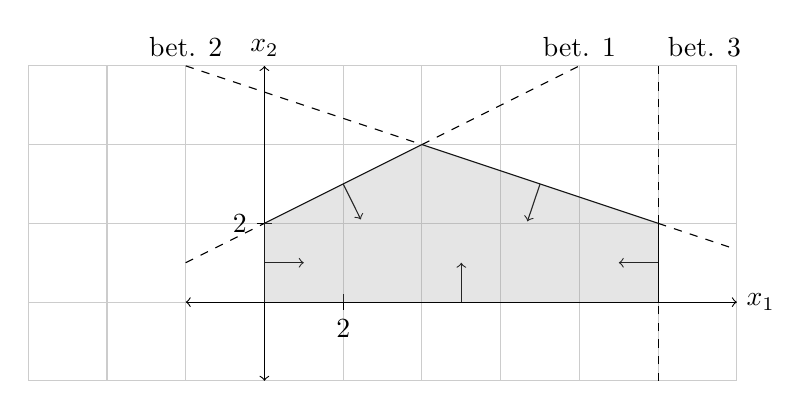
\begin{tikzpicture}
  %laver Grid. godt til når koordinater skal redigeres
  	\draw[thin,gray!40] (-3,-1) grid (6,3); 
  %x-aksen
  	\draw[<->] (-1,0)--(6,0) node[right]{$x_1$};
  	\draw[->] (2.5,0) -- (2.5,0.5);
  %y-aksen
  	\draw[<->] (0,-1)--(0,3) node[above]{$x_2$};
  	\draw[->] (0,0.5) -- (0.5,0.5);
  	
  %akse-markeringer
  	%\node[left] (xakse) at (0,1) {2};
  	\draw[] (-0.1,1) -- (0.1,1) node[pos=0,left] {2};
  	\draw[] (1,-0.1) -- (1,0.1) node[pos=0,below] {2};
  	
  %ligning 1
	\draw[domain=-1:0,variable=\x,dashed] 	plot({\x},{0.5*\x+1});
	\draw[domain=0:2,variable=\x] 			plot({\x},{0.5*\x+1});
	\draw[domain=2:4,variable=\x,dashed] 	plot({\x},{0.5*\x+1}) node[above] {bet. 1};
  	\draw[->] (1,1.5) -- (1.224,1.05);
	
  %ligning 2
  	\draw[domain=-1:2,variable=\x,dashed] 	plot({\x},{-(1/3)*\x+8/3}) node[above] at (-1,3) {bet. 2} ;
	\draw[domain=2:5,variable=\x] 			plot({\x},{-(1/3)*\x+8/3});
	\draw[domain=5:6,variable=\x,dashed] 	plot({\x},{-(1/3)*\x+8/3});
	\draw[->] (3.5,1.5) -- (3.34,1.026);

  %ligning 3
  	\draw[domain=-1:0,variable=\y,dashed] 	plot({5},{\y});
	\draw[domain=0:1,variable=\y] 			plot({5},{\y});
	\draw[domain=1:3,variable=\y,dashed] 	plot({5},{\y}) node[above right] {bet. 3};
	\draw[->] (5,0.5) -- (4.5,0.5);

  %løsningsmængden skraveret
	\fill[gray!80,nearly transparent] (0,0) -- (0,1) -- (2,2) -- (5,1) --(5,0) --  cycle;
\end{tikzpicture}
%	\captionof{figure}{Den mulige mængde af et standard maksimeringsproblem.}
%	\label{fig:maksprob2}
%\end{center}

\label{eks:maksprob2}
\end{eks}

\section{Løsninger til linære programmeringsproblemer}

Den mulige mængde er mængden af løsningsvektorer, $\vec{x}$, som opfylder alle problemets betingelser. Hvis en optimal løsning eksisterer vil denne derved være indeholdt i den mulige mængde.

\begin{defn}[Mulige løsninger og den mulige mængde]
En \textbf{mulig løsning} er en løsningsvektor $\vec{x}$, som opfylder alle problemets betingelser.\\
\textbf{Den mulige mængde} $\mathcal{F}$ er mængden af alle de mulige løsninger. Den vil derfor, for et standard maksimumsproblem være defineres som
\begin{align*}
\mathcal{F}=\{\vec{x} \in \mathds{R}^n|A\vec{x} \leq \vec{b}, \vec{x} \geq \vec{0}\}
\end{align*}
En vektor $\vec{x}^*$ kaldes en \textbf{optimal løsning}, hvis 
\begin{align}
	f(\vec{x}^*)=\max\limits_{\vec{x} \in \mathcal{F}}f(\vec{x}).
\end{align}
Et problem kaldes \textbf{inkonsistent} (usikker på oversættelse) hvis den mulige mængde er den tomme mængde, ellers er problemet \textbf{konsistent}. %Et problem kaldes \textbf{ubegrænset}, hvis objektfunktionen kan tage arbitrært store funktionsværdier for maksimeringsproblemer, og arbitrært små funktionsværdier for minimeringsproblemer. Ellers kaldes problemet \textbf{begrænset}.
\end{defn}
%Linje efter align og \\ skal enten skrives i bindende tekst eller gøres mere præcis

Den optimale løsning kan findes på forskellige måder heriblandt med simplex-metoden, som beskrives i senere kapitler. En anden måde er ved geometrisk visualisering af den mulige mængde. Denne metode er mulig for problemer med op til 3 variable, da løsningsmængden derved visualiseres som et plot i det tilsvarende antal dimensioner. 

\begin{eks}[Den mulige mængde]
Ved at indtegne betingelserne i et koordinatsystem, er det muligt at visualisere den mulige mængde som fællesmængden af de mængder, der dannes ud fra betingelserne. På Figur \ref{fig:maksprob2} er den mulige mængde for problemet i Eksempel \ref{eks:maksprob2} indtegnet. Der er desuden tegnet en pil for hver betingelse, som viser for hvilken side af linjen, at koordinaterne opfylder betingelsen. Den mulige mængde er farvet grå.

\begin{center}
	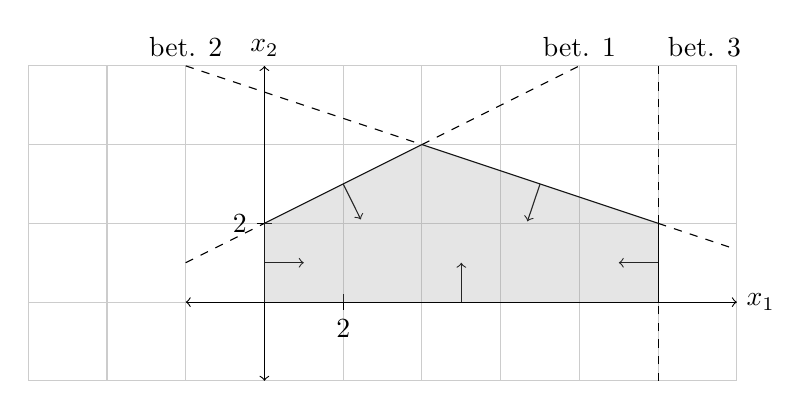
\begin{tikzpicture}
  %laver Grid. godt til når koordinater skal redigeres
  	\draw[thin,gray!40] (-3,-1) grid (6,3); 
  %x-aksen
  	\draw[<->] (-1,0)--(6,0) node[right]{$x_1$};
  	\draw[->] (2.5,0) -- (2.5,0.5);
  %y-aksen
  	\draw[<->] (0,-1)--(0,3) node[above]{$x_2$};
  	\draw[->] (0,0.5) -- (0.5,0.5);
  	
  %akse-markeringer
  	%\node[left] (xakse) at (0,1) {2};
  	\draw[] (-0.1,1) -- (0.1,1) node[pos=0,left] {2};
  	\draw[] (1,-0.1) -- (1,0.1) node[pos=0,below] {2};
  	
  %ligning 1
	\draw[domain=-1:0,variable=\x,dashed] 	plot({\x},{0.5*\x+1});
	\draw[domain=0:2,variable=\x] 			plot({\x},{0.5*\x+1});
	\draw[domain=2:4,variable=\x,dashed] 	plot({\x},{0.5*\x+1}) node[above] {bet. 1};
  	\draw[->] (1,1.5) -- (1.224,1.05);
	
  %ligning 2
  	\draw[domain=-1:2,variable=\x,dashed] 	plot({\x},{-(1/3)*\x+8/3}) node[above] at (-1,3) {bet. 2} ;
	\draw[domain=2:5,variable=\x] 			plot({\x},{-(1/3)*\x+8/3});
	\draw[domain=5:6,variable=\x,dashed] 	plot({\x},{-(1/3)*\x+8/3});
	\draw[->] (3.5,1.5) -- (3.34,1.026);

  %ligning 3
  	\draw[domain=-1:0,variable=\y,dashed] 	plot({5},{\y});
	\draw[domain=0:1,variable=\y] 			plot({5},{\y});
	\draw[domain=1:3,variable=\y,dashed] 	plot({5},{\y}) node[above right] {bet. 3};
	\draw[->] (5,0.5) -- (4.5,0.5);

  %løsningsmængden skraveret
	\fill[gray!80,nearly transparent] (0,0) -- (0,1) -- (2,2) -- (5,1) --(5,0) --  cycle;
\end{tikzpicture}
	\captionof{figure}{Skravering af den mulige mængde for et standard maksimeringsporblem.}
	\label{fig:maksprob2}
\end{center}

\end{eks}

\subsection{Niveaukurver}
Niveaukurver dannes ved fastsættelsen af en funktionsværdi $z=\vec{c}^T \vec{x}$. Niveaukurven er derved mængden af alle vektorer $\vec{x}$, som løser ligningen. Da målet er at maksimere $z$, er målet at finde den største $z$ for hvilken niveaukurven har en ikke-tom skæring med den mulige mængde. 

En løsningsvektor $\vec{x}$ kan omskrives til summen af en vektor parallel med $\vec{c}$, kaldet $\vec{x}_p$, og en vektor orthogonal med $\vec{c}$, kaldet $\vec{x}_o$. Her gælder det derved at, $\vec{x}_p=k\cdot \vec{c}$ for en skalar $k$, og at $\vec{x}_o^T \vec{c}=0$. Dette er muligt, da vektorrummet der er orthogonalt med $\vec{c}$ har dimension $n-1$, mens rummet dannet af $\vec{c}$ har dimension $1$. Da vil vektorrummet dannet af summen af disse rum have dimension $n$, da de to rum er orthononale. Derved kan alle løsningsvektorer $\vec{x}$ udtrykkes som summen af en vektor fra hvert af de to rum.

\begin{align*}
	f(\vec{x}) & \ = \ \vec{c}^T\vec{x}\\
	f(\vec{x_p}+\vec{x_o}) & \ = \
	\vec{c}^T\vec{x_p}+\vec{c}^T\vec{x_o} \ = \ 
	\vec{c}^T\vec{x_p} \ = \ 
	k\cdot \vec{c}^T\vec{c} \ = \ 
	k \○cdot \Vert \vec{c} \Vert ^2
\end{align*}
Da funktionsværdien derved er lig $k \cdot \Vert \vec{c} \Vert ^2$ gælder det derved om at maksimere $k$ for maksimeringsproblemer og at minimere $k$ for minimeringsproblemer. 


Dette kan ses i Eksempel \ref{eks:maksprob3}.
\begin{comment}
Bør niveaukurve defineres????? Hvordan kan dette bruges, for at finde $z$ er egentlig bare en omskrivning, så der mangler noget argumentation for at $z$ bliver større jo længere væk fra origo man er, hvilket giver ret god mening, men er svært at argumentere for uden at starte på geometri, så måske hele dette afsnit skulle flyttes, måske skal alt om løsninger skal flyttes til geometri?
\end{comment}


\begin{eks}[Optimal løsning fundet grafisk]
Niveaukurverne $46=\vec{c}^T \vec{x}$ og $25=\vec{c}^T \vec{x}$ er på Figur \ref{fig:maksprob3} indtegnet for programmeringsprogblemet fra Eksempel \ref{eks:maksprob2}.

	\begin{center}	
		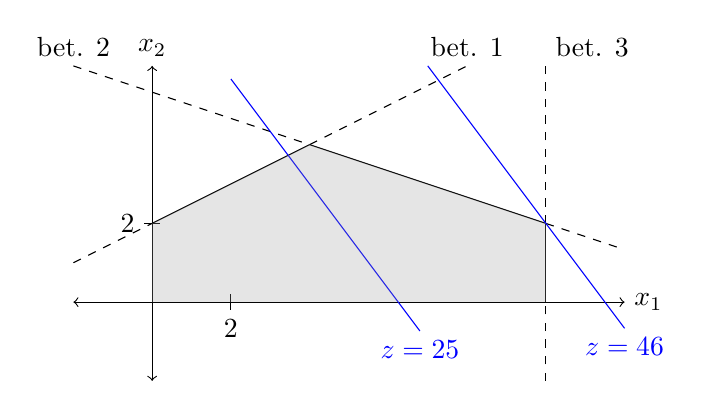
\begin{tikzpicture}
  %laver Grid. godt til når koordinater skal redigeres
  	%\draw[thin,gray!40] (-3,-1) grid (6,3); 
  %x-aksen
  	\draw[<->] (-1,0)--(6,0) node[right]{$x_1$}; 
  %y-aksen
  	\draw[<->] (0,-1)--(0,3) node[above]{$x_2$};
  	
  %akse-markeringer
  	%\node[left] (xakse) at (0,1) {2};
  	\draw[] (-0.1,1) -- (0.1,1) node[pos=0,left] {2};
  	\draw[] (1,-0.1) -- (1,0.1) node[pos=0,below] {2};
  	
  %ligning 1
	\draw[domain=-1:0,variable=\x,dashed] 	plot({\x},{0.5*\x+1});
	\draw[domain=0:2,variable=\x] 			plot({\x},{0.5*\x+1});
	\draw[domain=2:4,variable=\x,dashed] 	plot({\x},{0.5*\x+1}) node[above] {bet. 1};
	
  %ligning 2
  	\draw[domain=-1:2,variable=\x,dashed] 	plot({\x},{-(1/3)*\x+8/3}) node[above] at (-1,3) {bet. 2} ;
	\draw[domain=2:5,variable=\x] 			plot({\x},{-(1/3)*\x+8/3});
	\draw[domain=5:6,variable=\x,dashed] 	plot({\x},{-(1/3)*\x+8/3});
	

  %ligning 3
  	\draw[domain=-1:0,variable=\y,dashed] 	plot({5},{\y});
	\draw[domain=0:1,variable=\y] 			plot({5},{\y});
	\draw[domain=1:3,variable=\y,dashed] 	plot({5},{\y}) node[above right] {bet. 3};
	
  %niveaukurver
  	\draw[domain=3.5:6,variable=\x,blue] plot({\x},{-(4/3)*\x+23/3}) node[below] {$z=46$};
  	\draw[domain=1:3.4,variable=\x,blue] plot({\x},{-(4/3)*\x+25/6}) node[below] {$z=25$};
  	
  %c-vektor
  	%\draw[->,thick,red] (0,0) -- (2,1.5);

  %løsningsmængden skraveret
	\fill[gray!80,nearly transparent] (0,0) -- (0,1) -- (2,2) -- (5,1) --(5,0) --  cycle;
\end{tikzpicture}
		\captionof{figure}{Optimal løsning i den mulige mængde fundet som skæring med ligningen $z=46$.}
		\label{fig:maksprob3}
	\end{center}
	
På figuren ses det, at den største funktionsværdi $z=46$ findes i skæringen mellem bibetingelse 2 og 3.
Ved at løse bibetingelse 2 og 3 som 2 ligninger med 2 ubekendte findes det at den optimale løsning er $\vec{x}=\rvect{10 & 2}^T.$
\label{eks:maksprob3}
\end{eks}

\begin{comment}
Ved ikke om det giver mening under niveaukurver, at beskrive:
At da f er lineær, medfører det at den har en monoton udvikling når variablene har en monoton udvikling, så derfor hvis kurven rykkes ud fra en retnings vektor der står vinkelret på kurven, brude $Z$ være voksende eller aftagende. Og så gælder det om at finde den længst mulige vinkelrette afstand fra niveau kurven og origo, før at nivuae kurven ikke skære med den muligeløsningsmængde længere. Men ved ikke om det kan gøres strengent nok, synes bare som det er at niveau kurve afsnittet flagre lidt.
\end{comment}


\begin{comment}
Stadig to do i afsnittet\\
%- infeasible og unbounded tilfælde\\
%- niveaukurver\\
- Hvis der findes en løsning, findes der en optimal løsning (med evt. bevis. burde ikke være så svært med modstrid)\\
	%Men hører nok til nede i geometri afsnittet

Skal jeg have det med at løsninger findes i hjørner? det virker til at kræve en smule mere geometri og hører nok bedre til i geometri afsnittet. %Enig

%Er det standard maksimum problem eller standard maksimeringsproblem?
\end{comment}
